% ===
%
% Official LaTeX thesis template of the
% Chair for AI Methodology (AIM)
% RWTH Aachen University, Aachen, Germany
%
% Author: Jakob Bossek (bossek@aim.rwth-aachen.de)
% 
% AIM website: https://aim.rwth-aachen.de/
%
% ===

% AVAILABLE OPTIONS:
% ===
% thesis: either 'master' or 'bachelor' (all lowercase without quotation marks
\documentclass[thesis=bachelor]{AIM_thesis}

% includes/preamble.tex is the right place to add new packages etc.
% tables
\RequirePackage{booktabs}
\RequirePackage{colortbl}
\RequirePackage{multicol}
\RequirePackage{multirow}
\RequirePackage{xspace}
\RequirePackage[final]{pdfpages}

% pseudo-code
\usepackage[vlined, linesnumbered, ruled]{algorithm2e}
\SetKwComment{Comment}{/* }{*/}
\SetKwInput{KwData}{Input}
\SetKwInput{KwResult}{Output}
\IncMargin{1.5em}

% quotation
\RequirePackage{csquotes}

% bibliography
\RequirePackage[backend=biber,style=apa,natbib=true,sorting=nyt]{biblatex}

% \smiley{} and \frowney{}
\RequirePackage{wasysym}

% dummy text
\usepackage{blindtext}


% import commenting macros
%% commenting macros

% use this to hide larger blocks of material:
\usepackage{xcolor}
\usepackage{amsmath,amssymb}

% Define colors for authors
\definecolor{janecolor}{rgb}{0.2,0.6,0.6}
\definecolor{johncolor}{rgb}{0,0.7,0}

% Define colors for general macros
\definecolor{todocolor}{rgb}{0.9,0.1,0.1}
\definecolor{changedcolor}{rgb}{0.42,0.27,0.57}
\definecolor{addedcolor}{rgb}{0.867,0.176,0.361}

% General comment macro
\newcommand{\nbc}[3]{
    {\colorbox{#3}{\bfseries\sffamily\scriptsize\textcolor{white}{#1}}}
    {\textcolor{#3}{\sf\small$\blacktriangleright$\textit{#2}$\blacktriangleleft$}}
}
  
% Define individual comments for authors
\newcommand{\jane}[1]{\nbc{Jane}{#1}{janecolor}}
\newcommand{\john}[1]{\nbc{John}{#1}{johncolor}}

% Define general helper macros
\newcommand{\todo}[1]{\nbc{TODO}{#1}{todocolor}}
\newcommand{\changed}[1]{\nbc{CHANGED}{#1}{changedcolor}}
\newcommand{\added}[1]{\nbc{ADDED}{#1}{addedcolor}}

\newcommand{\redacted}[1]{\emph{[anonymized for review]}}
%\renewcommand{\redacted}[1]{#1}

% Use this to temporarily hide reviewing comments, todos, etc.:
%  \renewcommand{\jane}[1]{}
%  \renewcommand{\john}[1]{}

% Use this to make "changed" items appear normal:
%\renewcommand{\changed}[1]{#1}
%\renewcommand{\added}[1]{#1}
%\renewcommand{\todo}[1]{}

%% end commenting macros


% thesis title (pay attention to correct line-breaks)
\title{Advancing the State of the Art of Automated Artificial\\Intelligence~(AutoAI) by Evolutionary Computation:\\
A Preliminary Study in the Context of Hyper-Parameter Optimisation}
\author{Jane Doe}

% add supervisors
\supervisors{
Dr.~Jakob Bossek\\
Prof. Dr. Holger H. Hoos\\
}
% your student identifier (ID)
\id{123456}
% your e-mail address 
\email{jane.doe\@rwth-aachen.de}

% your address (not used at the moment)
% \street{Theaterstraße 35-39}
% \zip{52064}
% \city{Aachen}
% \country{Germany}

% source file(s) with bibliography entries
\addbibresource{bib.bib}

\begin{document}

% NOTE: DO NOT EDIT THE FOLLOWING LINES!

% title-page
\maketitle

\cleardoublepage
\pagenumbering{roman}

% abstract
\abstract{\blindtext}

% table of contents
\cleardoublepage
\pagestyle{empty}
\tableofcontents

% lists (comment out if not applicable)
\addcontentsline{toc}{chapter}{List of Figures}
\listoffigures
\addcontentsline{toc}{chapter}{List of Tables}
\listoftables
\addcontentsline{toc}{chapter}{List of Algorithms}
\listofalgorithms

% change page numbering style
\cleardoublepage
\pagenumbering{arabic}
\pagestyle{fancyplain}

% NOTE: ADD YOUR CONTENT HERE
%!TEX root=../main.tex
\chapter{Introduction}
\label{chap:introduction}

\blindtext[5]

\chapter{Guidelines}
\label{chap:guidelines}

We use the \LaTeX{} package \texttt{biblatex} for citations. Sample citation:~\cite{HutterEtAl2009}. You can also use full citations: \fullcite{HBPSTK2021TSPnormalization}

You are free to use British, American, Canadian or Australian English, but whatever you choose should be used consistently.
As Europeans, we recommend the use of British English (which is also well supported by spell and grammar checkers).

\section{Figures and tables}

Figure~\ref{fig:sample_image} shows a sample image, Table~\ref{fig:sample_table} shows an exemplary table and Algorithm~\ref{alg:sample_algorithm} shows some pseudo-code. Use the \texttt{booktabs} package to design nice tables. Avoid vertical lines whenever possible. We recommend to take a look at the presentation \href{https://people.inf.ethz.ch/markusp/teaching/guides/guide-tables.pdf}{Small Guide to Making Nice Tables} by Markus P\"uschel.

\begin{figure}
    \centering
    \includegraphics[width=0.3\textwidth]{example-image-a}
    \caption{Sample image.}
    \label{fig:sample_image}
\end{figure}

\begin{table}
  \centering
    \renewcommand{\tabcolsep}{4pt}
    \renewcommand{\arraystretch}{1.1}
    \begin{tabular}{ccrrrrrr}
    \toprule
    \multirow{2}{*}{\textbf{TSP Set}} & \multirow{2}{*}{\textbf{Mutation}} & \multicolumn{2}{c}{\bfseries RTS\textsuperscript{*}} & \multicolumn{2}{c}{\bfseries FR\textsuperscript{\dag}} & \multicolumn{2}{c}{\bfseries PAR10} \\
    \cmidrule(l{2pt}r{2pt}){3-4} \cmidrule(l{2pt}r{2pt}){5-6} \cmidrule(l{2pt}r{2pt}){7-8}
     &  & \textbf{EAX} & \textbf{LKH} & \textbf{EAX} & \textbf{LKH} & \textbf{EAX} & \textbf{LKH}\\
    \midrule
    RUE & - & 1.26 & 0.74 & 0.00 & 0.00 & 1.26 & 0.74\\
    \midrule
    Easy for & simple & 1.34 & 912.78 & 0.00 & 0.20 & 1.34 & 7\,608.11\\
    \cmidrule{2-8}
    EAX & sophistic. & 0.97 & 830.80 & 0.00 & 0.22 & 0.97 & 8\,230.61\\
    \midrule
    Easy for & simple & 117.97 & 0.74 & 0.00 & 0.00 & 117.97 & 0.74\\
    \cmidrule{2-8}
    LKH & sophistic. & 67.90 & 0.88 & 0.00 & 0.00 & 67.90 & 0.88\\
    \bottomrule
    \multicolumn{8}{l}{\textsuperscript{*} RTS: Running time of successful runs, \textsuperscript{\dag} FR: Failure ratio}\\%
\end{tabular}
    \caption{Sample table taken from~\cite{BossekKN00T19TSPcreative}.}
    \label{fig:sample_table}
\end{table}

\begin{algorithm}
\caption{Sample algorithm with the \texttt{algorithm2e} package.}
\label{alg:sample_algorithm}
\KwData{fitness function $f$, number of bits $n$, population size $\mu$}
\KwResult{Final population.}
Initialise a population $P$ of $\mu$ solutions each uniformly at random\;
\While{termination condition not met}{
  Select a parent $x \in P$ uniformly at random\;
  Generate $y$ from $x$ by bit-wise independent mutation flipping each bit with probability $\frac{1}{n}$\;
  Set $P = P \cup \{y\}$\;
  Let $x' = \text{argmin}_{x \in P} f(x)$\;
  Set $P = P \setminus \{x'\}$\;
} % While
\end{algorithm}

\section{Additional macros}

It is often useful to comment on different things while writing a report, adding ToDos or highlight changed or added parts. To this end the file \texttt{includes/commenting.tex} defines some useful macros.
\begin{itemize}
    \item Use \verb|\todo{...}| to add a ToDo:\newline \todo{Do this, do that}
    \item Use \verb|\changed{...}| to indicate changes:\newline \changed{This text was changed.}
    \item Use \verb|\added{...}| to highlight additions:\newline \added{This text was added.}
\end{itemize}

%!TEX root=../main.tex
\chapter{Conclusion}
\label{chap:conclusion}

\blindtext[5]


\printbibliography[heading=bibintoc, title=References]

\newpage
\pagestyle{empty}

\appendix

\chapter{Additional material}

\blindtext[5]

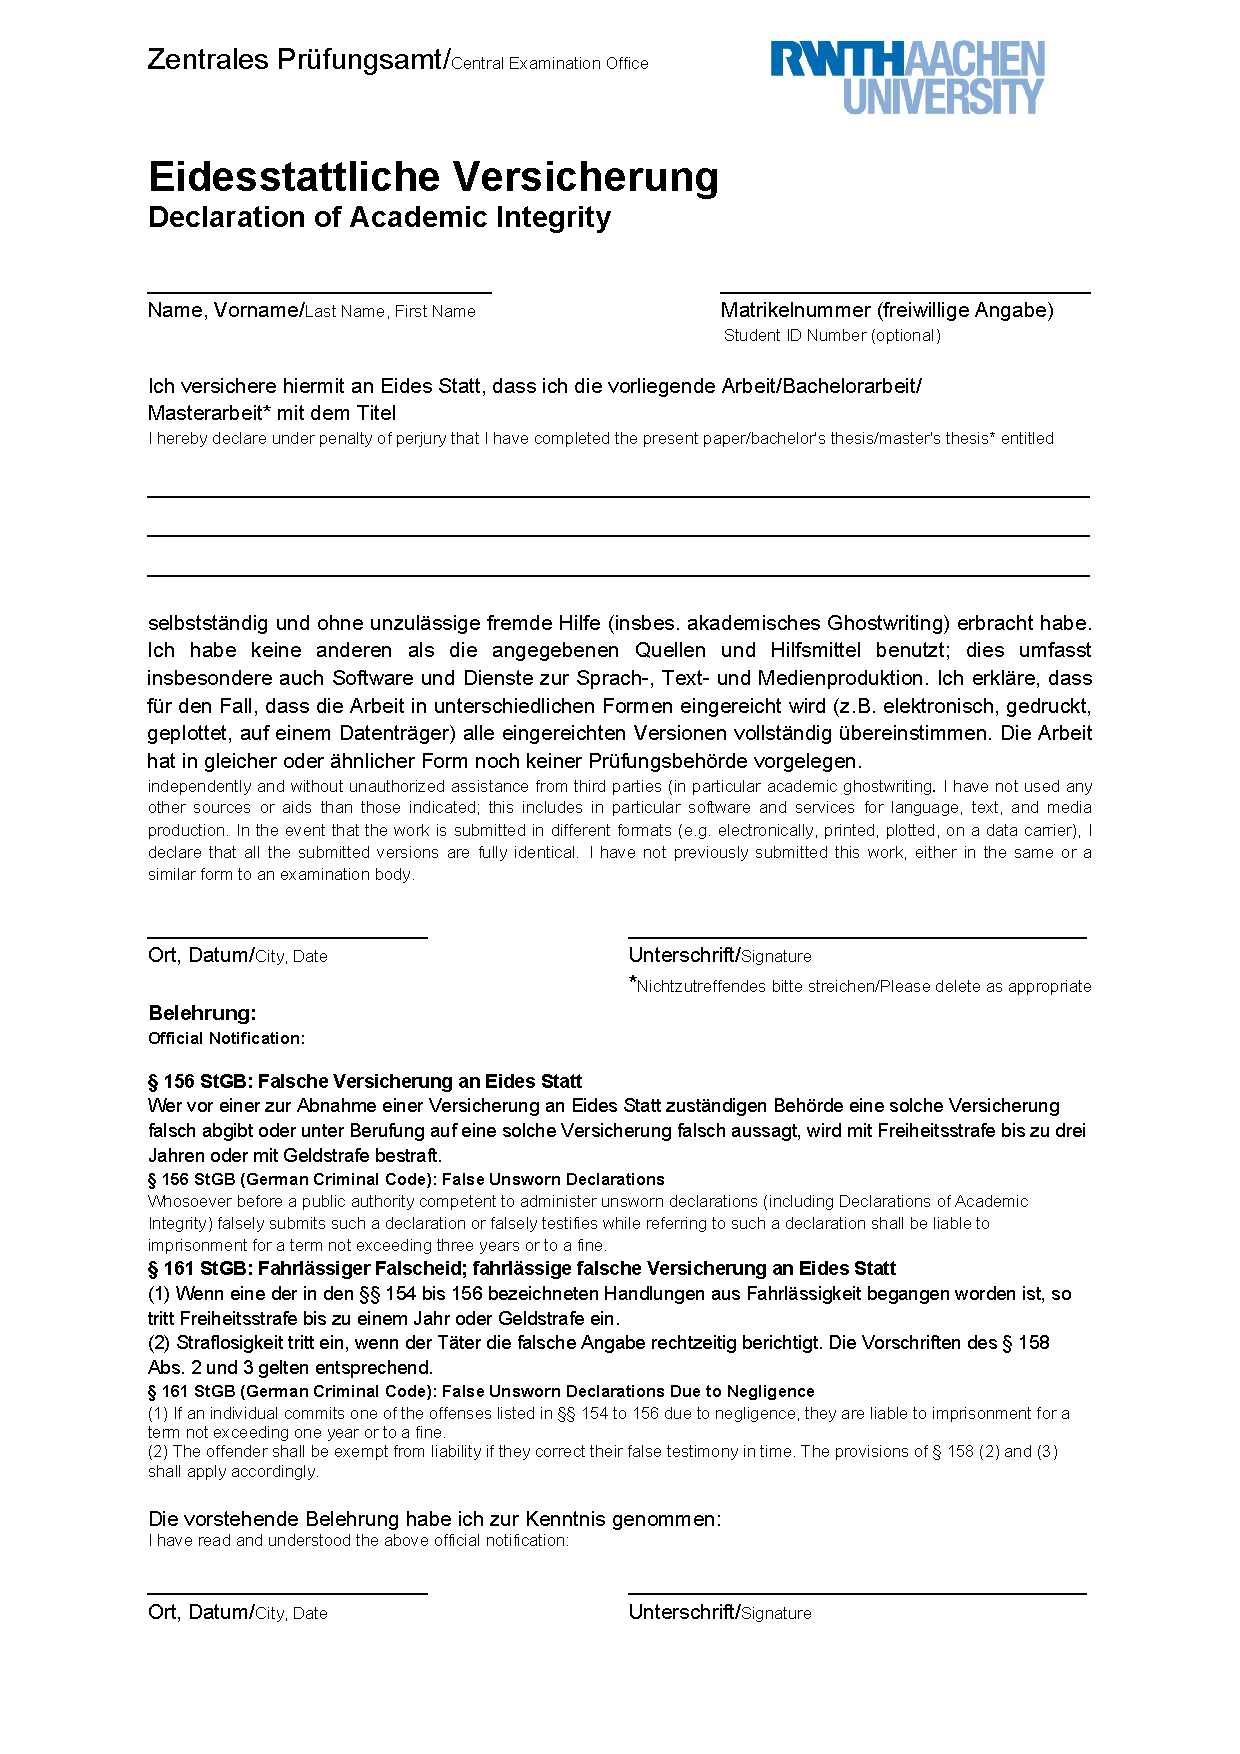
\includepdf[pages=-,pagecommand={},width=\textwidth]{files/oathstatement.pdf}

\end{document}
